\documentclass[sigconf,review]{acmart}

\usepackage{subcaption}
\usepackage{cleveref}

\crefname{figure}{Figure}{Figures}

\acmConference[SPLC'25]{29th International Systems and Software Product Line Conference}{September 01--September 05, 2025}{A Coruña, Spain}

\begin{document}

\title{On digital LEGO product lines for engineering education}

\author{Aleksandra Erohina}
\affiliation{
    \institution{University of Applied Sciences Upper Austria}
    \department{School of Engineering}
    \city{Wels}
    \state{Upper Austria}
    \country{Austria}
}

\author{Georg Hackenberg}
\orcid{0000-0003-3913-4148}
\affiliation{
    \institution{University of Applied Sciences Upper Austria}
    \department{School of Engineering}
    \city{Wels}
    \state{Upper Austria}
    \country{Austria}
}
\email{georg.hackenberg@fh-ooe.at}

\begin{abstract}
    TODO
\end{abstract}

\keywords{LEGO}

\maketitle

\section{Introduction}
\label{sec:introduction}

TODO~\cite{Hackenberg_2023} TODO~\cite{Baldwin_2023}

\paragraph{Research objective}

TODO

\paragraph{Research question}

Can we use digital LEGO for building interesting use cases for product line engineering that work well in engineering education?
Can we see typical issues in product line engineering such as module incompatibility in these use cases?
Can we use existing tools for digital LEGO modeling to build up relevant use cases already today?

\paragraph{Contribution}

TODO

\section{Related work}
\label{sec:related-work}

TODO

\section{Case study}
\label{sec:case-study}

In this third chapter we introduce the case study, which we have prepared for testing the viability of digital LEGO for product line engineering education.
In the following, we first provide an overview of the selected product line and its product variants in Section~\ref{sec:product-variants}.
Then, we introduce the atomic modules of the product line, from with the individual variants have been assembled in Section~\ref{sec:atomic-modules}.
Finally, we explain the configuration options of the drone use case in the form of a feature tree model in Section~\ref{sec:configuration-options}.

\subsection{Product variants}
\label{sec:product-variants}

\cref{fig:product-variants} provides an overview of the product variants for the drone use case.
The use case comprises three product variants, an ultra-light drone (see \cref{fig:ultra-light}), a free-style drone (see \cref{fig:free-style}), and a long-range drone (see \cref{fig:long-range}).

\begin{figure*}[htbp]
    \subcaptionbox{Ultra-light variant\label{fig:ultra-light}}{
        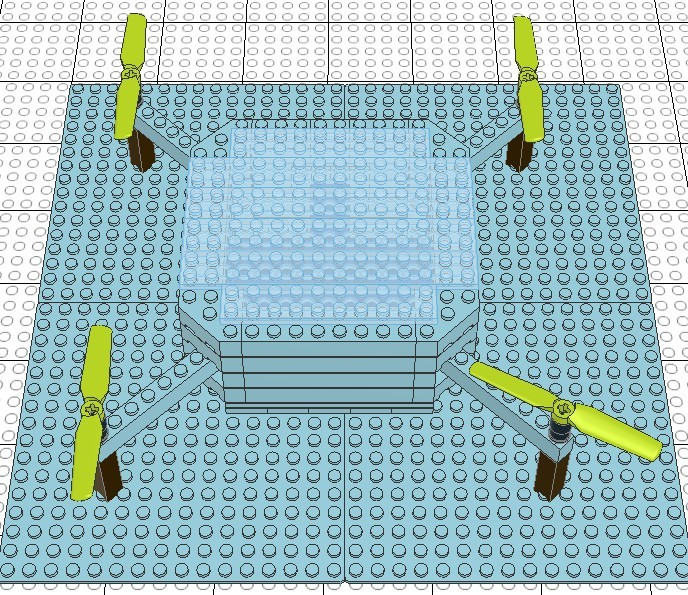
\includegraphics[height=4.4cm]{./drone-case-final-ultralight.jpg}
    }
    \hfill
    \subcaptionbox{Free-style variant\label{fig:free-style}}{
        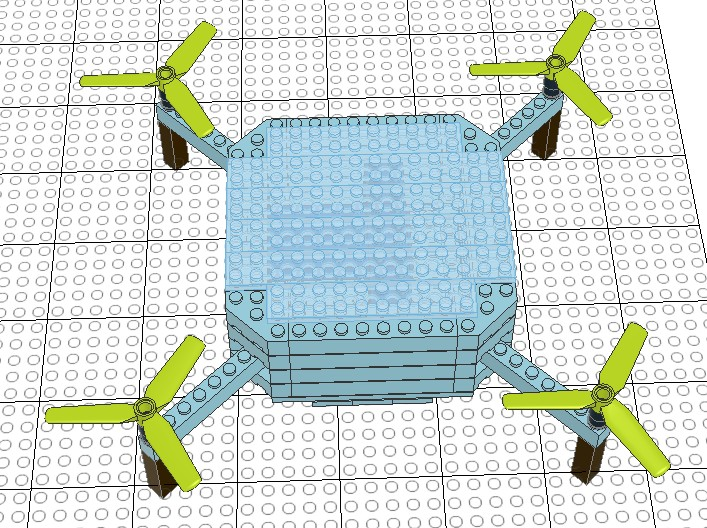
\includegraphics[height=4.4cm]{./drone-case-final-freestyle.jpg}
    }
    \hfill
    \subcaptionbox{Long-range variant\label{fig:long-range}}{
        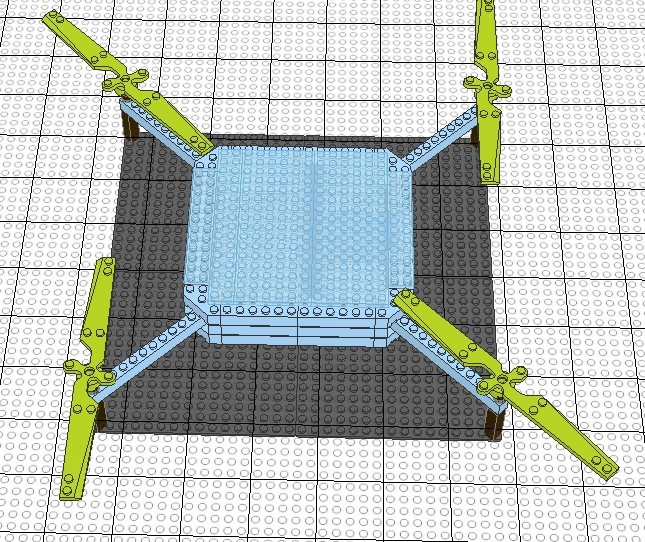
\includegraphics[height=4.4cm]{./drone-case-final-longrange.jpg}
    }
    \caption{Overview of the product variants for the drone use case.}
    \label{fig:product-variants}
\end{figure*}

\subsection{Atomic modules}
\label{sec:atomic-modules}

Each drone is made up of four modules, that deliver a certain function. 
Each module has its own variants, which makes it possible to offer a greater variety of products. 

\begin{figure*}[htbp]
    \subcaptionbox{Small frame\label{fig:frame-small}}{
        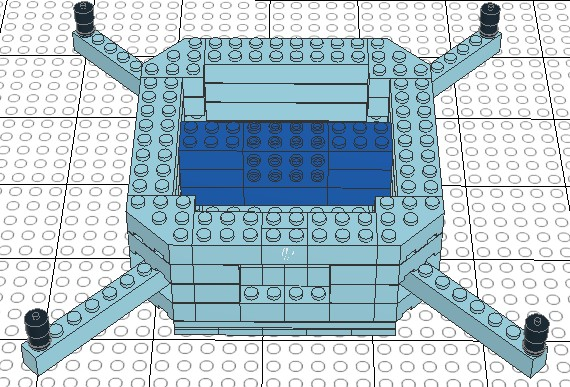
\includegraphics[height=2.3cm]{./drone-case-modules-frame-small.jpg}
    }
    \hfill
    \subcaptionbox{Large frame\label{fig:frame-large}}{
        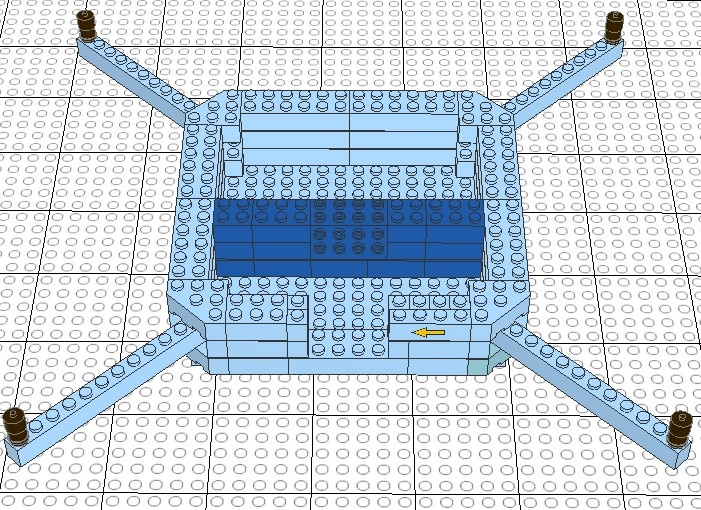
\includegraphics[height=2.3cm]{./drone-case-modules-frame-large.jpg}
    }
    \hfill
    \subcaptionbox{Small battery\label{fig:battery-small}}{
        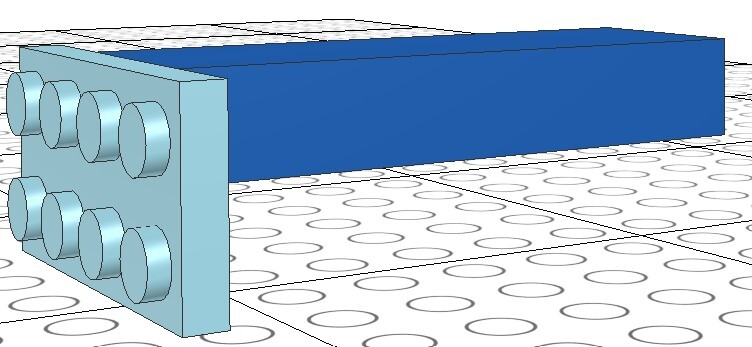
\includegraphics[height=1.3cm]{./drone-case-modules-battery-small.jpg}
    }
    \hfill
    \subcaptionbox{Medium battery\label{fig:battery-medium}}{
        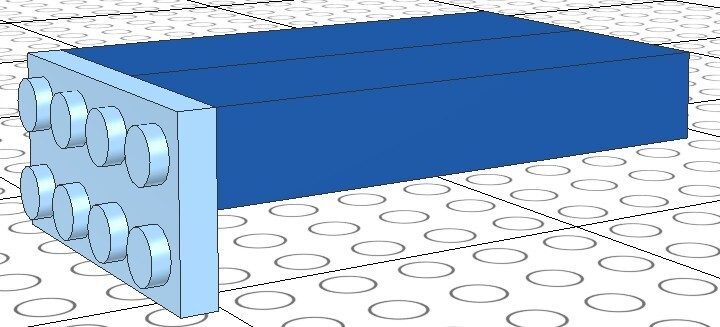
\includegraphics[height=1.3cm]{./drone-case-modules-battery-medium.jpg}
    }
    \hfill
    \subcaptionbox{Large battery\label{fig:battery-large}}{
        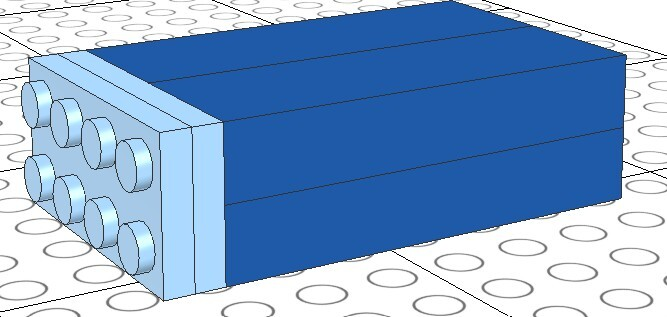
\includegraphics[height=1.3cm]{./drone-case-modules-battery-large.jpg}
    }
    
    \subcaptionbox{Small cover\label{fig:cover-small}}{
        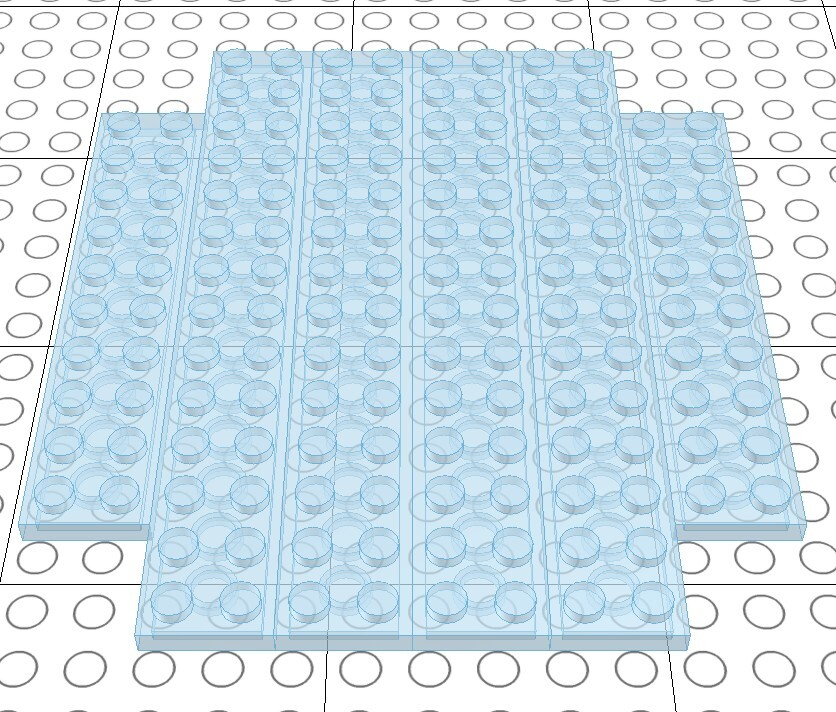
\includegraphics[height=2.3cm]{./drone-case-modules-cover-small.jpg}
    }
    \hfill
    \subcaptionbox{Large cover\label{fig:cover-large}}{
        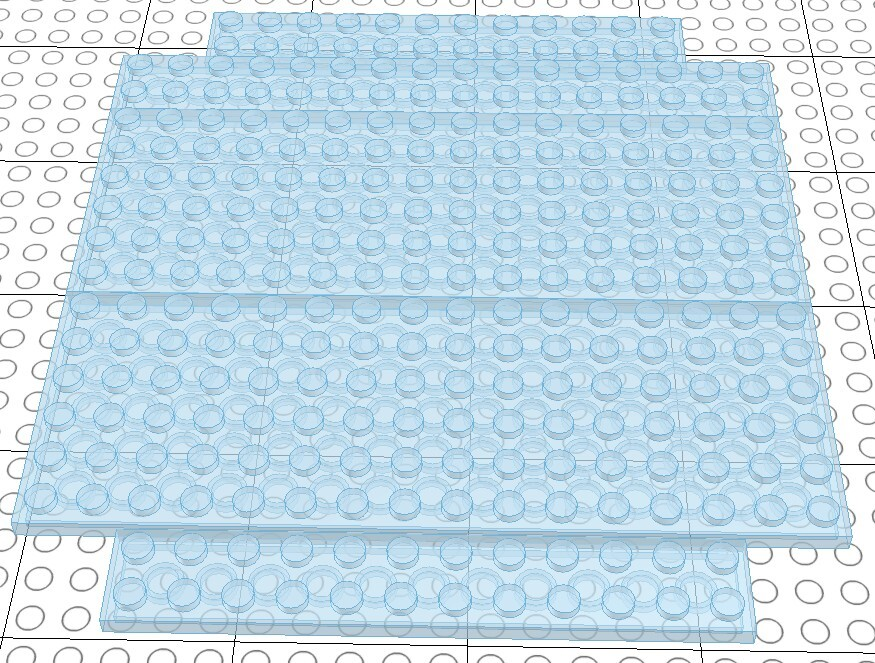
\includegraphics[height=2.3cm]{./drone-case-modules-cover-large.jpg}
    }
    \hfill
    \subcaptionbox{Small propellor\label{fig:propellor-small}}{
        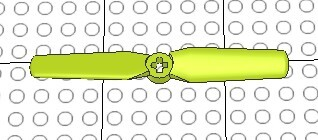
\includegraphics[height=1.5cm]{./drone-case-modules-propellor-2-small.jpg}
    }
    \hfill
    \subcaptionbox{Medium propellor\label{fig:propellor-medium}}{
        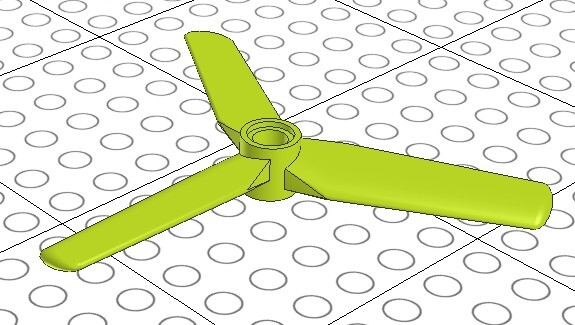
\includegraphics[height=1.5cm]{./drone-case-modules-propellor-3.jpg}
    }
    \hfill
    \subcaptionbox{Large propellor\label{fig:propellor-large}}{
        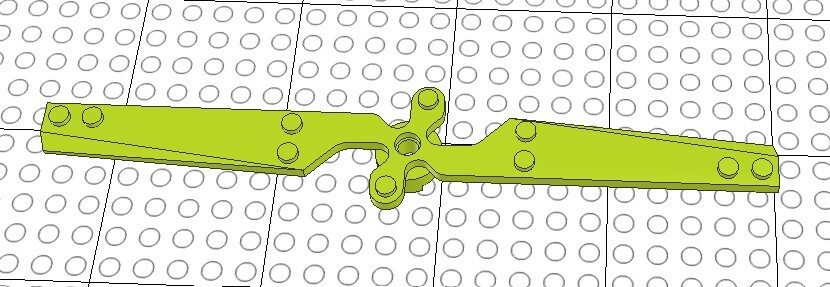
\includegraphics[height=1.5cm]{./drone-case-modules-propellor-2-large.jpg}
    }

    \caption{Overview of the atomic modules for the drone use case.}
    \label{fig:atomic-modules}
\end{figure*}

\subsubsection{Propellors}
\label{sec:propellors}

Propellers generate thrust by spinning rapidly, allowing a drone to move in all directions. 
A two-blade propeller provides better efficiency and longer flight times, while a triblade propeller offers more stability and maneuverability. 
Smaller propellers provide better agility, while bigger ones provide more thrust and efficiency, allowing the drone fly longer distances. 
However, larger propellers also require more power to spin.

\subsubsection{Batteries}
\label{sec:batteries}

A battery provides power for the drone to operate. 
A smaller capacity battery is lighter and more compact, which can improve the agility and maneuverability of the drone. 
However, smaller batteries have shorter flight times, which means that for longer flights a higher capacity battery is more suitable.

\subsubsection{Frames}
\label{sec:frames}

Frames serve as the structure that holds all the other parts together. 
A small frame is more maneuverable and agile, while a large frame offers more space for additional components (e.g. larger batteries).

\subsubsection{Covers}
\label{sec:covers}

Covers protect internal components of the drone, help to improve aerodynamics and serve an aesthetic purpose as well.

\subsection{Configuration options}
\label{sec:configuration-options}

TODO \cref{fig:feature-tree}

\begin{figure*}[htbp]
    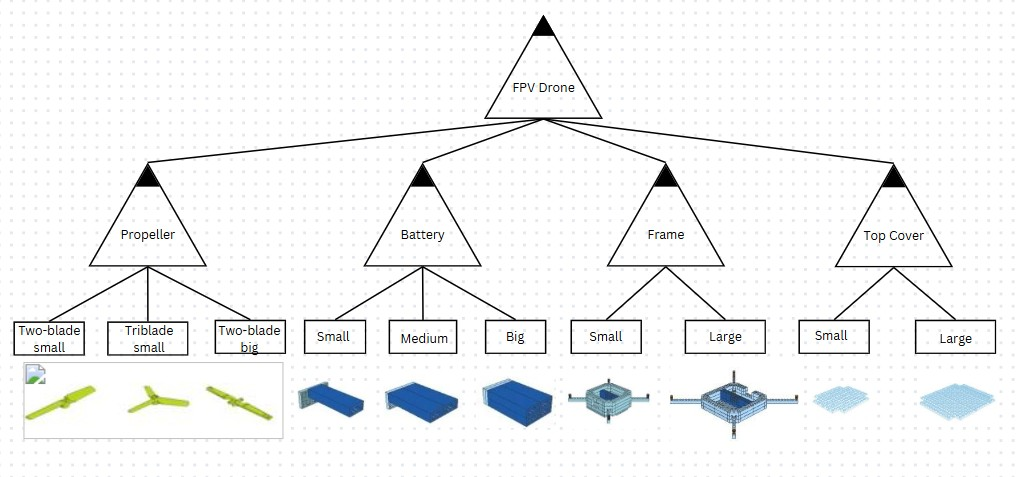
\includegraphics[width=\textwidth]{./drone-case-feature-tree.jpg}
    \caption{Overview of the configuration options for the drone use case.}
    \label{fig:feature-tree}
\end{figure*}

The modules can be combined to design customized end products.  For that purpose, the FPV drone variability model is developed. 
When a customer wishes to design and buy a drone, multiple decisions have to be made before the final system can be build. 
Figure 3 shows that the variation points Propeller, Battery, Frame and Cover have a mandatory dependency with the FPV drone, which means that they have to be included in the final product. 
For each of these variation points a variant has to be selected. The variants are connected by an alternative choice dependency with a minimum and maximum equal to one, which means that only one variant has to be chosen to be included to the final product. 
Additionally, two types of constraint dependencies exist: require constraint and exclude constraint. The require constraint means that when the small frame is selected, the small cover should be integrated to the system, and when the large frame is selected, the large cover should be integrated. 
The excluding constraint means that when a large propeller is selected, the small frame can not be integrated to the design and this relationship goes the other way round as well.


Physical interfaces between interacting modules enable their geometric connection. A frame for the drone example has three interfaces: with a battery, with propellers and with a cover. 
However, several geometrical constraints should be considered. These include:

•	Size and shape constraints: Modules must be designed in such a way that they can physically fit together without interference. 
For the drone example, the large frame can accommodate all three types of batteries, while the small frame is limited to only small and medium batteries because of the size constraints.

•	Alignment constraints: Modules must be aligned properly to ensure proper functioning when assembled together. 
For example, covers must be oriented correctly relative to frames to serve the protective and aesthetic purposes. 

•	Interference constraints: It is important to consider potential interferences between modules, such as conflicting shapes or components that may impede proper assembly or operation. 
It is technically feasible to install any propeller on any frame, but practical constraints come into play. For instance, a large propeller cannot be mounted on a small frame without interference, as it would collide with the frame during rotation.
These geometric restrictions cause constraint dependencies that are shown in Figure 3.


\section{Conclusion}
\label{sec:conclusion}

TODO

\bibliography{main}
\bibliographystyle{ACM-Reference-Format}

\end{document}